% Chapter Template

\chapter{Power Efficiency Analysis} % Main chapter title

\label{Chapter6} % Change X to a consecutive number; for referencing this chapter elsewhere, use \ref{ChapterX}

\lhead{Chapter 6. \emph{Power Efficiency Analysis}} % Change X to a consecutive number; this is for the header on each page - perhaps a shortened title

%----------------------------------------------------------------------------------------
%	SECTION 1
%----------------------------------------------------------------------------------------

\section{Introduction}
The current implementation of the SWAN WEAR allows us to choose which way we want to process the data from the smartwatch application:
\begin{itemize}
 \item Perform minimum amount of computation on the watch and just send values to be processed by the SWAN PHONE application
 \item Send the expression to SWAN WEAR application for evaluation
\end{itemize}

Typically, the recommended approach is to minimize the computation on the watch to save battery, but in certain cases,  when the expression does not require frequent evaluation, we might get better power savings if we choose to perform the evaluation on the watch.

\section{Design}
Before proceeding to the data analysis, according to the GQM\cite{gqm_1}\cite{gqm_2} paradigm, we should define the goal, the questions and the metrics.
    Our goal is to analyse the power consumption of phone and smartwatch, for the purpose of comparing two different methods of acquiring sensor data
    with respect to differences in power consumption of the phone and the smartwatch, in context of the SWAN android application.

\textbf{Question 1}: What is the overhead of gathering data from the smartwatch, compared to running evaluation on the watch?
\begin{itemize}
  \item Metric 1:  Battery level on Android Phone
  \item Metric 2:  Battery level on Android Smartwatch
  \item  Metric 3:  Expression runtime in seconds
\end{itemize}

\textbf{Question 2}:  What is the overhead of gathering data from the test sensor\footnote{Test Sensor is our reference implementation of SWAN sensor} compared to the real hardware sensor?
\begin{itemize}
 \item Metric 1:  Battery level on Android Phone
 \item Metric 2: Battery level on Android Smartwatch
 \item  Metric 3:  Expression runtime in seconds
\end{itemize}

\section{Experiment Planning}
\subsection{Context Selection}
The experiment will be run on the simulated(laboratory) environment, composed of Android Phone and Android Wear Smartwatch. We will consider our experiment as a real life problem because:
\begin{itemize}
 \item The tests are performed on real devices, which are used as reference for many Android developers
 \item The test suite is composed of various sensor data, which reflect the actual SWAN performance in real life applications.
\end{itemize}

\subsection{Variable Selection}

The main dependent variable is the power consumption expressed as battery power consumed during the experiment.
The independent variables are data acquisition method and delay.
Data acquisition methods  have two options:
\begin{itemize}
 \item Phone based SWAN expressions
 \item Wear based SWAN expressions
\end{itemize}

Delay is set by us, but to avoid spending too much time on experiment, we will choose between two options: fast (100ms) and slow (1 second).

\subsection{ Hypothesis Formulation}

    We consider $\mu$ the battery power consumed by the test suite. Since we have two devices to measure power consumption from, 
    $\mu$ will be calculated as $\delta$\textsubscript{phone} +  $\delta$\textsubscript{wear}, where $\delta$ is the difference in battery levels 
    before and after the experiment.
    
    Special case:\label{special_case} If the power consumption is better on the phone but worse on the watch for the given approach, we cannot test the hypothesis:
    \begin{itemize}
      \item ($\delta$ \textsubscript{wear test 1} - $\delta$ \textsubscript{wear test 2}) $\textgreater$ 0
      \item ($\delta$\textsubscript{phone test 1} - $\delta$\textsubscript{phone test 2}) $\textless$ 0 
    \end{itemize}
    
    The reason why we can't apply our hypotheses is because the smartwatch and the phone have different hardware, idle power consumption and 
    battery installed. We cannot compare them directly, but we can claim that one approach is better for the  phone but worse for the watch and let the developers
    make decision on what they want to value the most: phone or watch battery.

    \textbf{Question 1:} What is the overhead of gathering data from smartwatch, compared to running evaluation on the watch? \newline
Conjecture(P): There is a difference between gaining data and evaluating expression on the smartwatch \newline
Consequence(Q): The difference between only gaining data and evaluating expression on the smartwatch is significant. \newline
\textit{Null hypothesis} - No observable difference in power consumption between only gathering data and evaluating expression on the watch \newline
H0: ( $\mu$\textsubscript{phone based} - $\mu$\textsubscript{wear based} = 0) \newline
  Alternative hypothesis - There is a difference in power consumption between only gaining data on watch and running a SWAN expression on the watch \newline
H1:($\mu$\textsubscript{phone based} - $\mu$\textsubscript{wear based} $\neq$ 0)  \newline

    \textbf{Question 2:}  What is the overhead of gathering data from test sensor compared to real hardware sensor?\newline
    Conjecture(P): There is  a difference between using test sensor and real sensor on the smartwatch\newline
    Consequence(Q): The difference between only gaining data and evaluating expression on the smartwatch is significant.\newline
    \textit{Null hypothesis} - No observable difference in power consumption between using test sensor and hardware sensor on the watch\newline
H0: ($\mu$\textsubscript{test} - $\mu$\textsubscript{real} = 0)\newline
    Alternative hypothesis - There is a difference in power consumption between using test sensor and hardware sensor on the watch\newline
H1:($\mu$\textsubscript{test} - $\mu$\textsubscript{real} $\neq$ 0)\newline

\subsection{Subject Selection}
For this experiment we will use a batch of expressions targeting multiple sensors available on the smartwatch.
The batch for phone based tests contains the following expressions:
\begin{itemize}
 \item \begin{verbatim}self@wear_movement:x?delay={$delay}$server_storage=FALSE{ANY,0}\end{verbatim}
 \item \begin{verbatim}self@wear_gamerotation:x?delay={$delay}$server_storage=FALSE{ANY,0}\end{verbatim}
 \item \begin{verbatim}self@wear_linearacceleration:x?delay={$delay}$server_storage=FALSE{ANY,0}\end{verbatim}
 \item \begin{verbatim}self@wear_gravity:x?delay={$delay}$server_storage=FALSE{ANY,0}\end{verbatim}
 \item \begin{verbatim}self@wear_heartrate:heart_rate?delay={$delay}$server_storage=FALSE{ANY,0}\end{verbatim}
\end{itemize}

The batch for wear based expressions contains the following expressions:
\begin{itemize}
 \item \begin{verbatim}wear@movement:x?delay={$delay}$server_storage=FALSE{ANY,0}\end{verbatim}
 \item \begin{verbatim}wear@gamerotation:x?delay={$delay}$server_storage=FALSE{ANY,0}\end{verbatim}
 \item \begin{verbatim}wear@linearacceleration:x?delay={$delay}$server_storage=FALSE{ANY,0}\end{verbatim}
 \item \begin{verbatim}wear@gravity:x?delay={$delay}$server_storage=FALSE{ANY,0}\end{verbatim}
 \item \begin{verbatim}wear@heartrate:heart_rate?delay={$delay}$server_storage=FALSE{ANY,0}\end{verbatim}
\end{itemize}

The \textbf{\{\$delay\}} will be replaced by the appropriate value when registering an expression

To evaluate the performance of the real sensor compared to the  test sensor, we will run the test sensor for the same 
amount of values and we will compare its power consumption with power consumption from hardware sensors. 
There will be two implementations of the test sensor, one for each data acquisition approach.

\subsection{Experiment Design}
For the first part of the experiment we will have two factors to vary: \textbf{data acquisition approach} and \textbf{delay}.
This will give us four different scenarios to test:

\begin{center}
  \begin{tabular}{ |l|l|l|l| }
  \hline
  \multicolumn{4}{ |c| }{Factor A: Data acquisition Method} \\
  \hline
  \multicolumn{2}{|c|}{Phone Based Evaluation}  & \multicolumn{2} {|c|}{Wear Based Evaluation} \\
  \hline
  \multicolumn{2}{|c|}{Factor B: Delay}  & \multicolumn{2} {|c|}{Factor B: Delay} \\
  \hline
  Delay: 100ms & Delay: 1000 ms & Delay: 100ms & Delay: 1000 ms\\
  \hline
  3x Experiments & 3x Experiments & 3x Experiments &3x Experiments\\
  \hline
  \end{tabular}
\end{center}

The second part of the experiment will focus on quantifying the discrepancy between power consumption when using a test sensor
versus using a real, hardware sensor. In this test scenario we also apply delay of 100 ms and 1000ms, to be fully aware of the implications of all factors.

\begin{center}
 \textbf{Delay 100 ms:}
\end{center}

\begin{center}
  \begin{tabular}{ |l|l|l|l| }
  \hline
  \multicolumn{4}{ |c| }{Factor A: Data acquisition Method} \\
  \hline
  \multicolumn{2}{|c|}{Phone Based Evaluation}  & \multicolumn{2} {|c|}{Wear Based Evaluation} \\
  \hline
  \multicolumn{2}{|c|}{Factor B: Sensor Type}  & \multicolumn{2} {|c|}{Factor B: Sensor Type} \\
  \hline
  Real Sensor & Test Sensor & Real Sensor & Test Sensor\\
  \hline
  3x Experiments & 3x Experiments & 3x Experiments &3x Experiments\\
  \hline
  \end{tabular}
\end{center}

\begin{center}
 \textbf{Delay 1000 ms:}
\end{center}

\begin{center}
  \begin{tabular}{ |l|l|l|l| }
  \hline
  \multicolumn{4}{ |c| }{Factor A: Data acquisition Method} \\
  \hline
  \multicolumn{2}{|c|}{Phone Based Evaluation}  & \multicolumn{2} {|c|}{Wear Based Evaluation} \\
  \hline
  \multicolumn{2}{|c|}{Factor B: Sensor Type}  & \multicolumn{2} {|c|}{Factor B: Sensor Type} \\
  \hline
  Real Sensor & Test Sensor & Real Sensor & Test Sensor\\
  \hline
  3x Experiments & 3x Experiments & 3x Experiments &3x Experiments\\
  \hline
  \end{tabular}
\end{center}

\subsection{Threats to Validity}
External: The experiment is being performed on a specific setup. Even if the devices in our tests are chosen to represent the reference,
the Android market is fragmented, and different Android versions, hardware and smartwatches can yield to a different result

Internal: Basing our power consumption  results on battery levels increase the total error rate. Nonlinear discharge rate,
battery wear level\cite{battery_wear_proc} can influence the final conclusion. To avoid these battery limitations, we will perform tests only when the battery is fully charged, 
so the discharge pattern will be the same. Also to reduce the battery wear impact, the tests will be performed with limited time delay,
and without any phone or smartwatch usage between the tests.

 Internal: The batch execution of the expression can induce extra error if different types of sensors have different power consumption. 
 We will try to limit the impact of this error type by proving that the selection of the sensors has the same power draw by
 performing single sensor benchmark with initial full battery. 
 
 Internal: The communication using Bluetooth may vary energy consumption based on distance or obstacles between devices.
 We minimize the impact of Bluetooth, by placing phone and smartwatch in close proximity with no obstacles in between.
 
 External: Heart rate sensor can be unpredictable. In some circumstances, the heart rate sensor can stop giving values. 
 Since we were not wearing the smartwatch during our test, we placed it on the charging dock, with no charging cable connected and the phone
 in close proximity. By satisfying these conditions, the experiment setup and results can be verified.
 
 \subsection{Instrumentation}
 The following devices are available to perform our experiment:
 \begin{itemize}
  \item Phone - Nexus 6P - manufactured by Huawei,  with latest Android 6.0 Marshmallow installed and with Android security patch level: 1 June 2016. 
  \item Smartwatch - Motorola 360 gen 2, with latest Android 6.0 Marshmallow, android wear version 1.5 
 \end{itemize}

 We could have a bigger selection of phones to run SWAN on them, since we only have one smartwatch available,
 the different processors  and Bluetooth chips might induce more randomness in our observations.
 Besides we can argue that Nexus phones are used by default by lots of smartwatch manufacturers for tests.
 Before proceeding to experiment setup, the devices were factory reset and the only Android Wear app necessary for smartwatch connection was installed.
 We observed that by default a lot of Google applications are installed on the Nexus Phone. Some of them also have watch apps packaged.
 To avoid possible battery drain from other applications we decided to disable the following apps on the Nexus Phone:
 \begin{itemize}
  \item  Google Drive
  \item Google Play Games
  \item Google Play Music
  \item Hangouts
  \item Google Maps
  \item Google Photos
  \item Youtube
  \item Google Docs
 \end{itemize}

 Measuring power consumption of both approaches requires us to have accurate tools.
 The power consumption should be measured on both phone and Android Wear device, so we could better understand what are the pros and cons of using each method.
 We have two methods of measuring the power consumption:
 \begin{itemize}
  \item Using the Android battery starts, which provide the current power draw if the device is equipped with a hardware fuel gauge (Our test devices Nexus 6P and Moto 360 gen 2 )\cite{fuel_gauge}.
  \item The standard setup: Running each method for a prolonged amount of time and measure the battery level after the experiment is done.
 \end{itemize}

 Using the hardware power gauge is a very useful feature to measure the power consumption. Unfortunately, it suffers from two major disadvantages:
 \begin{itemize}
  \item We need to run another battery sensor, so the results may not reflect the constant power consumption of the SWAN application running.
  \item Hardware fuel gauge has its own limitations, and the computed power usage may not be accurate.
 \end{itemize}

 Using battery level measurement can also be affected by battery maximum capacity, charge-discharge cycle, but since we repeat the experiment for both options on the same hardware, and without delay we can argue that results can be compared.
 Additionally, measuring the battery levels allow us to have a better average value.
 
 \subsection{Experiment Execution}
 After initial research we concluded that the data from hardware fuel gauge is highly inaccurate on Android Wear.
 The reason is exceptionally power efficient hardware and a high error rate for the power consumption sensor. 
 Also we are unable to test what is the power implication of running the SWAN WEAR foreground service. 
 In order to obtain some power metrics, we will monitor battery levels on the phone and the smartwatch after the SWAN expression returns a given amount of sensor values, in both scenarios.
The results that we get will be analysed based on power consumption on both phone and smartwatch.
The experiment steps should be performed in the following order:
\begin{itemize}
 \item Factory reset both phone and smartwatch.
 \item Pair smartwatch to the phone.
 \item Install SWAN on the phone and smartwatch.
 \item Run a preliminary test, to see if SWAN is ready to operate.
 \item Charge both phone and smartwatch to 100\%.
 \item Install test application.
 \item Disable Wi-Fi and radio, leave only Bluetooth.
 \item Start test application and turn off the screen of the phone.
 \item Test application should take the phone and wear battery levels and remaining Power values before starting test evaluations.
 \item Wait for application to finish the test suite.
 \item Test application will take the battery levels and remaining power values after the tests are finished and will write them on local storage for further analysis.
 \item Repeat the experiment three times.
\end{itemize}

For the testing purpose, we will avoid sensors that are dependent of user motion to actually work: 
\begin{itemize}
 \item Step counter sensor - will send updates only if the user walked after the last query. It might also be related to hardware implementation of the sensor in our test device\cite{motorolla_stepcounter}. 
 \item Light sensor - the updates are triggered by changes in light level and since our test setup is configured to run for a long time, we cannot include a sensor triggered by external,
 undefined behaviour
\end{itemize}

Surprisingly, the Heart Rate Sensor will still give values even if it is not mounted on the wrist, so we can use it for our test purpose. 
The heart rate sensor is different compared to regular sensors found on the phone. The smallest granularity for heart rate results is one second,
so specifying a smaller delay will not make any sense.  Delays bigger than one second instead will be fulfilled by SWAN implementation.
Unfortunately, due to different delay, we could not prove that the heart rate sensor consumes the same amount of power as the rest of the sensors in the test suite.
We still provide our findings, but we will not include heart rate in power comparisons.
 
 \subsection{Preliminary Tests}
Preliminary tests shows us that we cannot rely on the estimated power reported by the fuel gauge sensors. In case of our phone device,
Nexus 6P, the reported values in Nano-watts were not accurate at all. Instead, the current discharge current was reported, 
but we can not use it in our tests, since it will interfere with our test setup.
We encountered the similar problem on our smartwatch, Motorola 360 generation 2. 
The reported value in Nano-watts was not corresponding with the maximum theoretical energy that the watch battery is able to hold, according to the specifications.

To get comparable results we are supposed to guarantee equal conditions for both test scenarios.
Since SWAN is quite power efficient and sensors that we are targeting are also very power efficient, the test should run for a long period of time.
We estimated that a notable difference in battery levels should occur after running SWAN expressions for around two hours' period.
Running tests for a longer period of time can help us identify even smaller differences, 
but the necessity of running the experiments with different types of expressions and also the number of repetitions for each scenario make use of longer runtimes prohibitive.
Also we should take into consideration the charging time necessary after each run of the experiment,
with smartwatch normally losing the highest battery percentage and having long recharge times.


\subsection{Test Application}
The test application was built in order to run tests in batch order and gather the battery level data. To avoid power consumption from external sources, such as phone screen, we implemented the testing code as foreground service\cite{foreground_service} which is not hibernated by the Android system when the screen is off. 
The testing application has the following workflow:
For each SWAN expression:
\begin{itemize}
 \item Register a SWAN expression and get the battery level of the phone before the experiment
 \item Register a SWAN expression and get the battery level of the smartwatch before the experiment
 \item Unregister SWAN expressions used to get the battery levels on phone and wear
 \item Register the start time
 \item Calculate the number of values necessary for the run, based on the given expected runtime in microseconds
 \item Register the experiment expressions and wait until the number of values are reached
 \item Register expression end time
 \item Get the battery level of the phone after the experiment
 \item Get the battery level of the smartwatch after the experiment
\end{itemize}


Once the tests for the expression are done, the application will write on local storage, in a text file the expressions name,
battery levels before and after, the number of values received and the total runtime.

Even if the program runs in a separate service, we are not allowed to block in the main thread. 
We are actually required to wait for the SWAN expression to terminate, so we sent the computation in another thread and use Latch\cite{latch} to wait for expression execution.

\section{Results}

We performed all experiments according to the Experiment Design and we obtained relevant data. To improve readability,
we decided not to include the raw data in this chapter. If you are interested to see the raw data, check \hyperref[AppendixPower]{Appendix A}, for tables containing the
average values of 3 experiments.

\subsection{Preliminary Analysis}

We present the results of our data in the graphs below.
The Figures 6.1-6.5 contain the data relevant for our hypothesis testing.
 
 \begin{figure}[htbp]
  \centering
    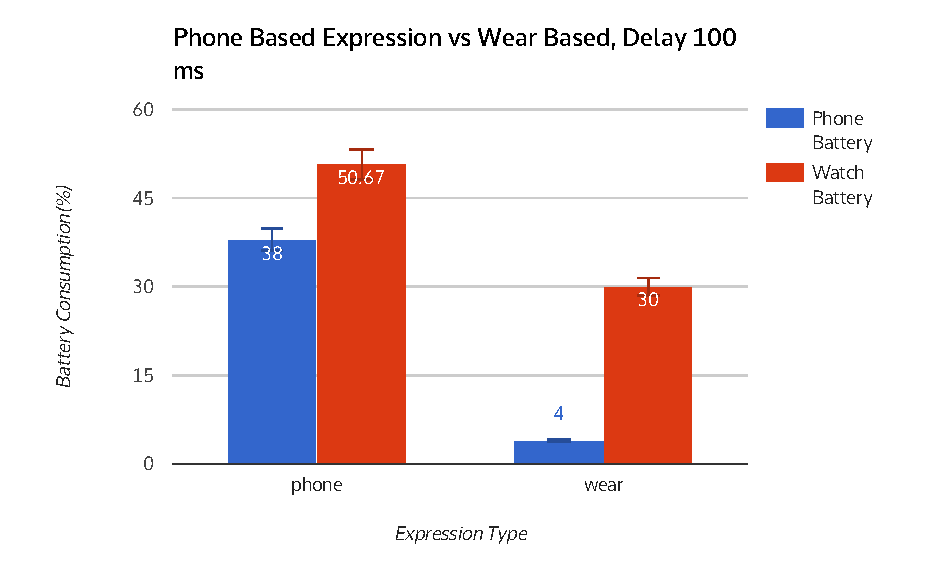
\includegraphics[scale=0.8]{Figures/phone_vs_wear_100.pdf}
    \rule{35em}{0.5pt}
  \caption[Phone vs Wear Based Expressions, delay 100 ms]{Phone vs Wear Based Expressions, delay 100 ms}
  \label{fig:phone_vs_wear_100}
\end{figure}

\hyperref[fig:phone_vs_wear_100]{Figure 6.1} represents the power consumption of phone based expressions and wear based expressions for very fast delay,
and fixed number of received values. As we can see the phone based SWAN expressions are highly inefficient, phone battery dropped \textbf{34\%} more and watch battery dropped 
\textbf{20 \% } more than watch based SWAN expression. 

 \begin{figure}[htbp]
  \centering
    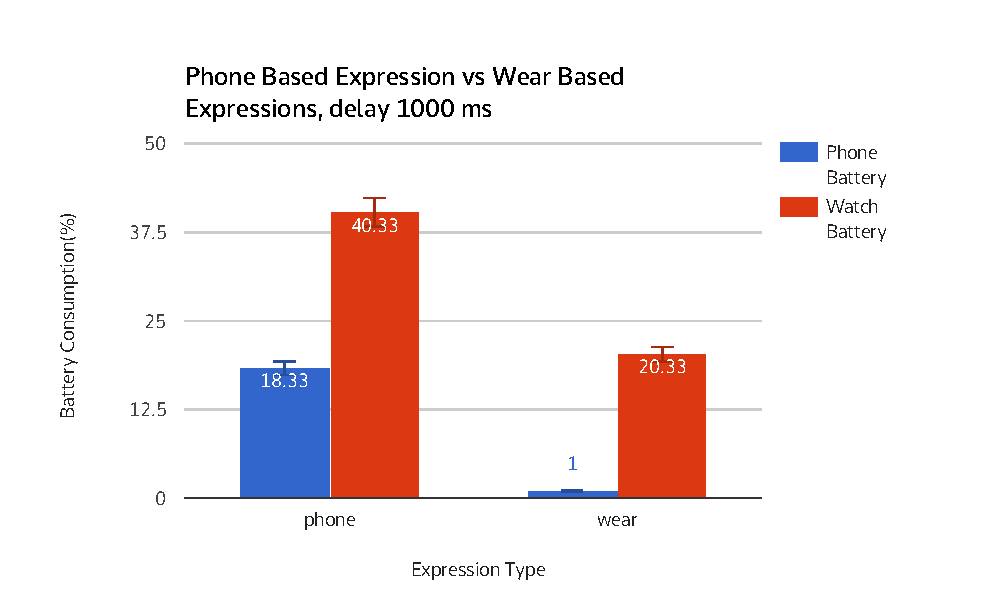
\includegraphics[scale=0.8]{Figures/phone_vs_wear_1000.pdf}
    \rule{35em}{0.5pt}
  \caption[Phone vs Wear Based  Expressions, delay 1000 ms]{Phone vs Wear Based  Expressions, delay 1000 ms}
  \label{fig:phone_vs_wear_1000}
\end{figure}

\hyperref[fig:phone_vs_wear_1000]{Figure 6.2} represents the power consumption of phone based expressions and wear based expression for normal delay, also
with fixed number of received values. This test scenario highlights the very good power savings for phone battery, with only \textbf{1\%} drop in phone battery for watch based SWAN
expressions. Phone based expressions perform better than in fast delay scenario, but still very power inefficient for both watch and phone.

 \begin{figure}[htbp]
  \centering
    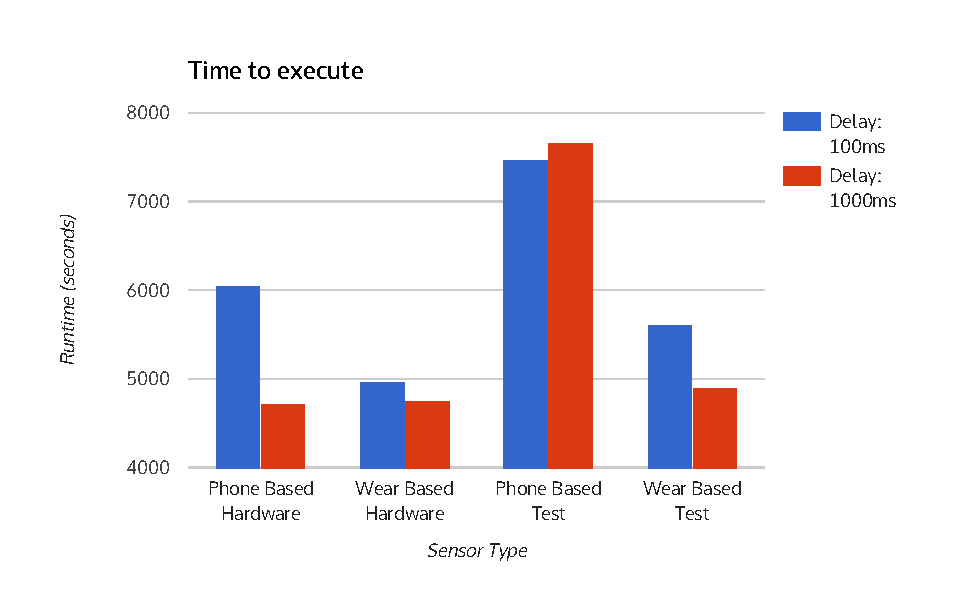
\includegraphics[scale=0.8]{Figures/execution_times.pdf}
    \rule{35em}{0.5pt}
  \caption[Run time of different number of sensors, baseline 4800 seconds]{Run time of different number of sensors, baseline 4800 seconds}
  \label{fig:execution_times}
\end{figure}

As part of the experiment, we noticed that different types of expression have different runtimes for the same number of recorded values. The expected runtime for all expressions,
given the delay, was 4800 seconds. \hyperref[fig:execution_times]{Figure 6.3} shows the execution times of wear and phone based expressions, for both real sensors and our software test sensor.
Longer runtimes translate into more battery consumption, but we will not take the run times into consideration, and we will focus on the fixed amount of values that our test application should receive.

 \begin{figure}[htbp]
  \centering
    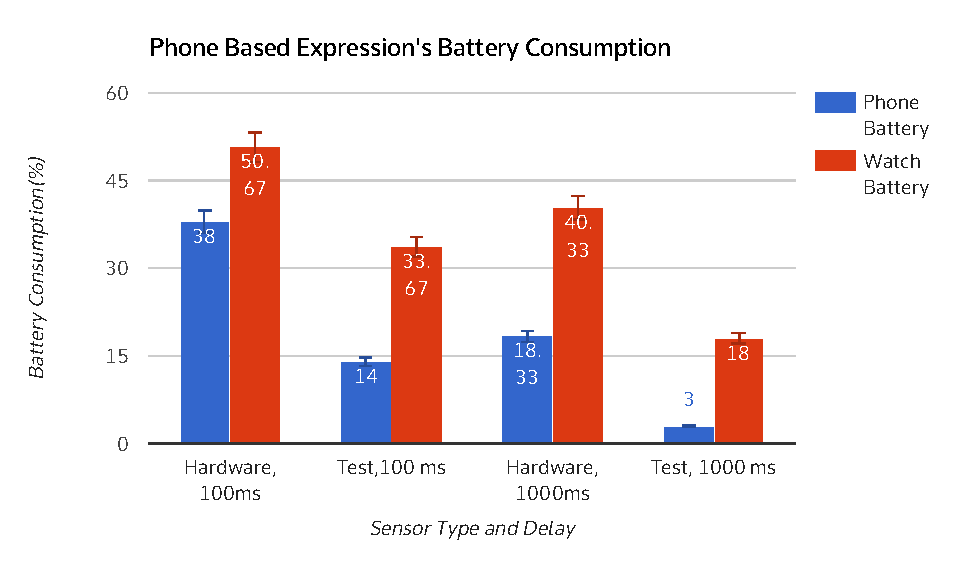
\includegraphics[scale=0.8]{Figures/phone_expr_consumption.pdf}
    \rule{35em}{0.5pt}
  \caption[Phone Based Expression Power Consumption]{Phone Based Expression Power Consumption}
  \label{fig:phone_expr_consumption}
\end{figure}

The graphs show clearly that phone based expressions are not efficient.  We should further validate our approach by excluding the variable update rate from a real hardware sensor.
Test sensor will always send updates with the specified delay, and as we can see in \hyperref[fig:phone_expr_consumption]{Figure 6.4}, the shorter delay from hardware sensor is responsible
for more power used.

 \begin{figure}[htbp]
  \centering
    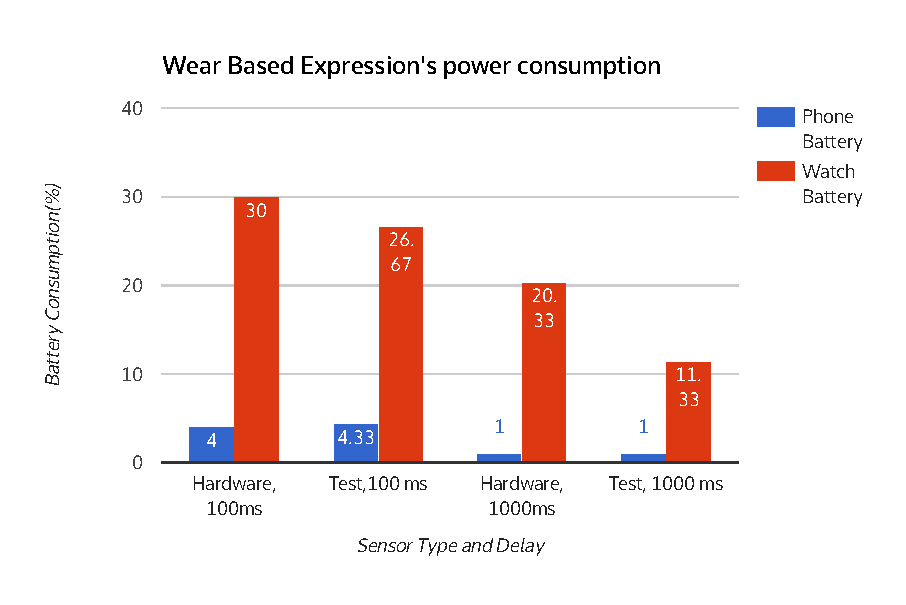
\includegraphics[scale=0.8]{Figures/wear_expr_consumption.pdf}
    \rule{35em}{0.5pt}
  \caption[Wear Based Expression Power Consumption]{Wear Based Expression Power Consumption}
  \label{fig:wear_expr_consumption}
\end{figure}

For watch based expressions, the phone battery improvements are non-existent(or, at least do not surpass our error threshold to be considered a difference). On the other hand,
a stable delay still translates into \textbf{ 5 to 10\%} less battery consumed on the watch as we can see in \hyperref[fig:wear_expr_consumption]{Figure 6.5}

\subsection{Hypothesis Testing}
After preliminary data analysis we notice that we don't have the \hyperref[special_case]{special case}, so we can proceed to test out hypothesis.

\textit{Research Question 1:} What is the overhead of gathering data from the smartwatch, compared to running evaluation on the watch? \newline
Following the formulas described in Hypothesis Formulation section, we observe that for delay of 100 ms, phone based expressions consume 
\textbf{34\% more} phone battery and \textbf{~20\% more } smartwatch battery. Taking into account the 5\% error by the imperfection of our instruments,
we reject the Hypothesis H0, and accept the Hypothesis H1, for the given delay of 100 ms.

For given delay of 1000ms, we observe that  phone based expressions consume 
\textbf{17\% more} phone battery and \textbf{~20\% more } smartwatch battery. Taking into account the 5\% error by the imperfection of our instruments,
we reject the Hypothesis H0, and accept the Hypothesis H1.

 \textit{Research Question 2:}  What is the overhead of gathering data from the test sensor compared to the real hardware sensor?\newline
Following our further research on why the phone based expressions consume so much power, we wanted to test the sensor update delay, as a factor
which increases the power consumption. Our test sensor implementation always honours the delay specified in the expression, compared to a very weak delay guarantee
given by a real hardware sensor.

For given delay of 100ms, hardware sensor consumed \textbf{14\% more} phone battery and \textbf{~17\% more } smartwatch battery than the test sensor, assuming that both test and hardware
sensor is implemented as phone based expression.
Taking into account the 5\% error by the imperfection of our instruments, we reject the Hypothesis H0 and accept the Hypothesis H1.

For given delay of 1000ms, hardware sensor consumed \textbf{15\% more} phone battery and \textbf{~22\% more } smartwatch battery than the test sensor, assuming that both the test and the hardware
sensor is implemented as phone based expression.
Taking into account the 5\% error by the imperfection of our instruments, we reject the Hypothesis H0 and accept the Hypothesis H1.

Comparing the wear based expressions is more complicated. We could not record any notable differences on the phone battery consumption during our tests, so we will focus on the smartwatch battery consumption.

For given delay of 100ms,  hardware based sensor consumed \textbf{3\% more} watch battery than the test sensor.
Our 5\% error rate requires to have a difference of at least 1.5\% in battery levels (5\% of 30\% battery drop is equal to 1.5\%). We
reject hypothesis H0 and accept Hypothesis H1.

For given delay of 1000ms,  hardware based sensor consumed \textbf{9\% more} watch battery than the test sensor.
Our 5\% error rate requires to have a difference of at least 1\% in battery levels (5\% of 20\% battery drop is equal to 1\%). We
reject hypothesis H0 and accept Hypothesis H1.

\section{Final Results Discussion}

After performing all the tests from our suite, we revealed that using the phone based expression in the current SWAN implementation is not a good idea.

Specifically, the phone is getting heated on low delays and the phone battery drop is one order of magnitude higher than using the SWAN expression evaluation on the watch.

After careful analysis we identified two possible reasons why the phone based expression consumes so much power, but also what can further improve the power consumption of smartwatch based expressions:
\begin{itemize}
 \item The hardware sensor does not honour the requested delay:
 \begin{itemize}
  \item A lot of values are being sent over Bluetooth and the phone has to drop them because they do not arrive in the given timestamp.
  \item Wear based expression drop values locally, so no extra values are sent over Bluetooth.
  \item Phone based test sensor show much better battery when the values arrive at given delay.
 \end{itemize}
 \item The SWAN's evaluation engine drops too many values that were supposed to be accepted\footnote{See Figure 6.6 and the explanation below}:
 \begin{itemize}
  \item The Bluetooth and synchronization delay changes the arrival time of the values, and the value-accept function takes into consideration arrival time, not the time when values were recorded.
  \item Test Sensor revealed poor performance of the accepting sensor value implementation, which translates two times longer runtimes than predicted in our test scenarios.
  \item Having the expected runtime as close as possible to real runtime can save battery.
 \end{itemize}
\end{itemize}

  \begin{figure}[htbp]
  \centering
    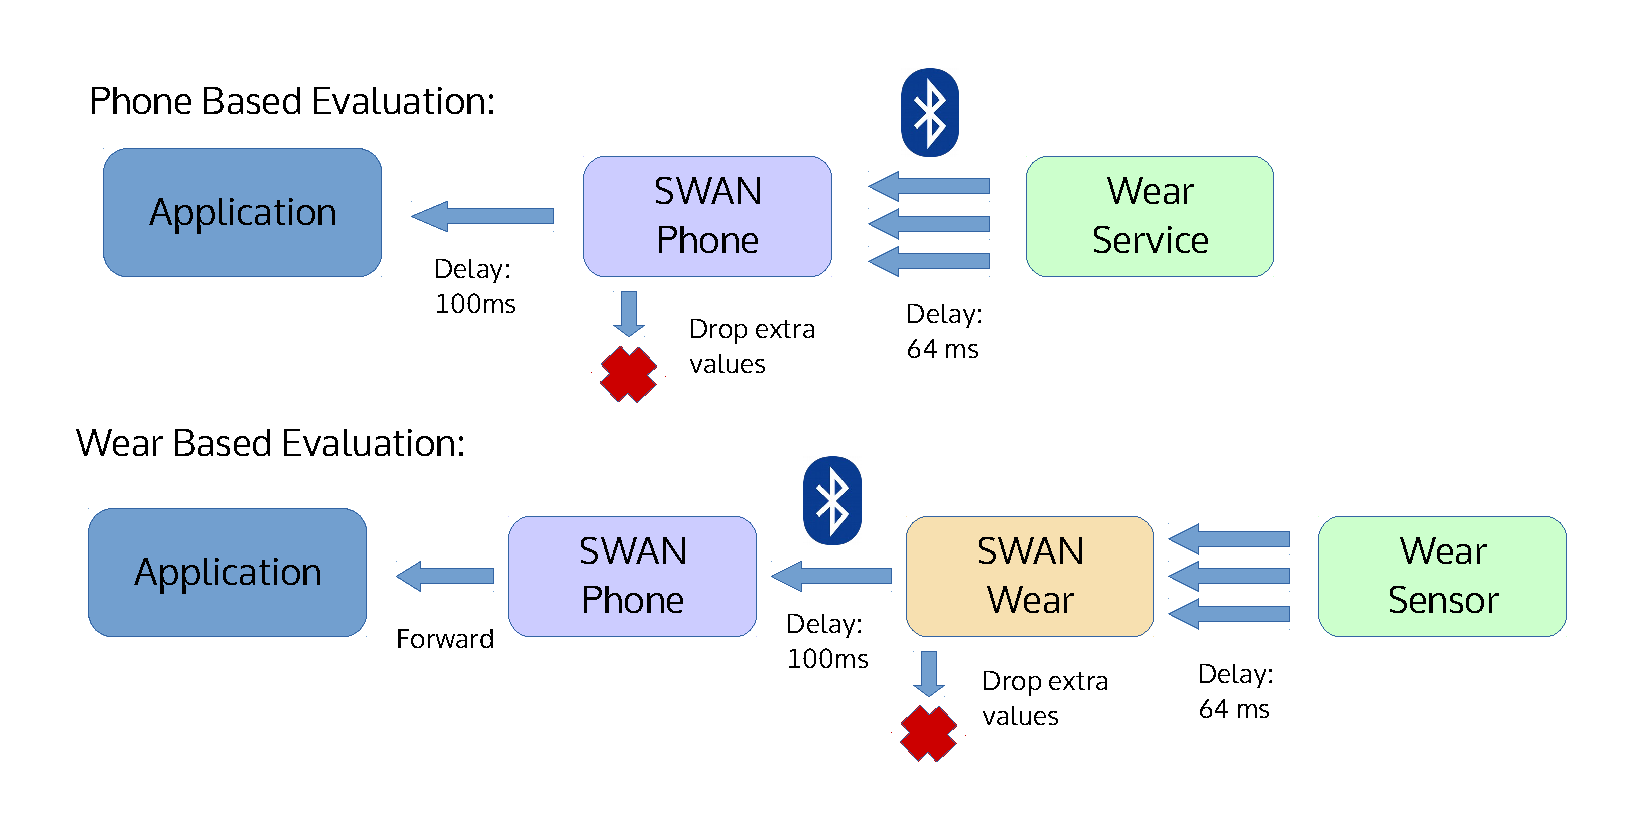
\includegraphics[scale=0.5]{Figures/swan_drop_val.pdf}
    \rule{35em}{0.5pt}
  \caption[Dropping values in Phone and Wear Based Expressions]{Dropping values in Phone and Wear Based Expressions}
  \label{fig:swan_drop_val}
\end{figure}

Furthermore, we noticed that hardware sensors will not enforce the delay and SWAN should take care about this. As we can see in \hyperref[fig:swan_drop_val]{Figure 6.6}, 
phone based approach will drop the values after they were sent through Bluetooth, while in the wear based expressions, values are dropped locally, which translates into less power consumption.
Even without the test sensor, some values are dropped because of the extra delay incurred by Bluetooth.

 The accept values implementation performance needs to be further investigated.
 As the result of our experiments we can conclude that the test sensor, with ideal delay, has lower battery consumption.
 The excessive runtime is a side effect on the test sensors, and log analysis(we record when the values are being dropped) give us some clues to the problem.
 We observe an increase in runtimes when a lot of values are dropped. However we didn't manage to fully isolate the
 problem so we could say for sure that the way SWAN enforces delay is responsible for long runtimes.


